\setcounter{chapter}{-1}
\chapter{Markdown标记语言}

%\begin{adjustwidth}{1cm}{1cm}
%\shadowbox{
%\begin{minipage}[l]{0.8\textwidth}
{\itshape
Markdown是一种轻量级标记语言,创始人为约翰・格鲁伯(John Gruber)。它允许人们“使用易读易写的纯文本格式编写文档,然后转换成有效的XHTML(或者HTML)文档”。

Markdown的目标是实现“易读易写”,成为一种适用于网络的书写语言。一份使用Markdown格式撰写的文件应该可以直接以纯文本发布,并且看起来不会像是由许多标签或是格式指令所构成。

Markdown的语法全由一些符号所组成,这些符号经过精挑细选,其作用一目了然。比如:在文字两旁加上星号,看起来就像强调。Markdown的列表看起来,嗯,就是列表。Markdown的区块引用看起来就真的像是引用一段文字,就像你曾在电子邮件中见过的那样。
}
%\end{minipage}
%}
%\end{adjustwidth}

\vspace{0.2in}
\noindent
一、实验要求
\begin{enumerate}
  \item 了解Markdown标记语言。
  \item 掌握Markdown基本语法。
  \item 使用Markdown撰写文档。
\end{enumerate}

\vspace{0.2in}
\noindent
二、实验准备
\begin{enumerate}
  \item 一台已安装有Windows操作系统或联网的计算机。
  \item 一个Markdown编辑器。
\end{enumerate}

\vspace{0.2in}
\noindent
三、实验内容

\vspace{0.1in}
(一)在线Markdown编辑器
\begin{itemize}
  \item \href{https://www.zybuluo.com}{Cmd Markdown(作业部落)}
  \item \href{https://maxiang.io}{马克飞象}
  \item \href{http://markdown.xiaoshujiang.com/}{小书匠}
  \item \href{https://stackedit.io/editor}{StackEdit}
  %\item \href{http://mahua.jser.me/}{MaHua}
\end{itemize}

\vspace{0.1in}
(二)Markdown基本语法
\begin{figure}[h]
  \centering
  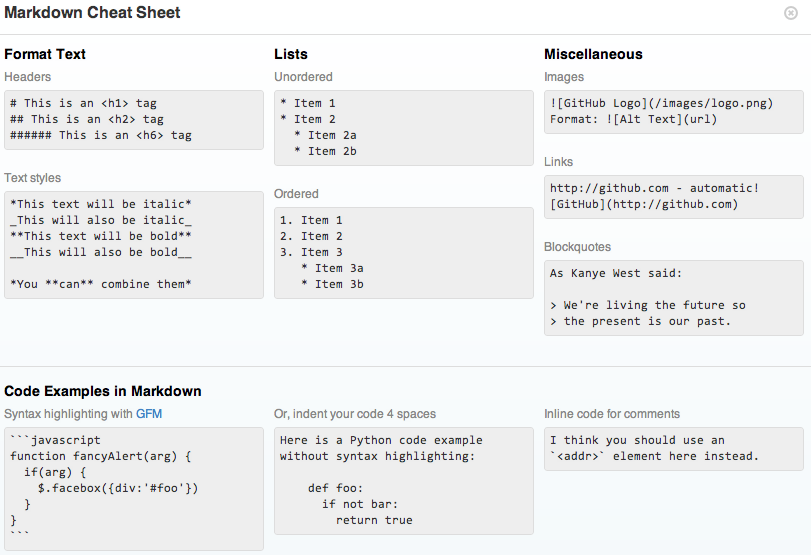
\includegraphics[width=\textwidth]{markdown_cheatsheet_01.png}
  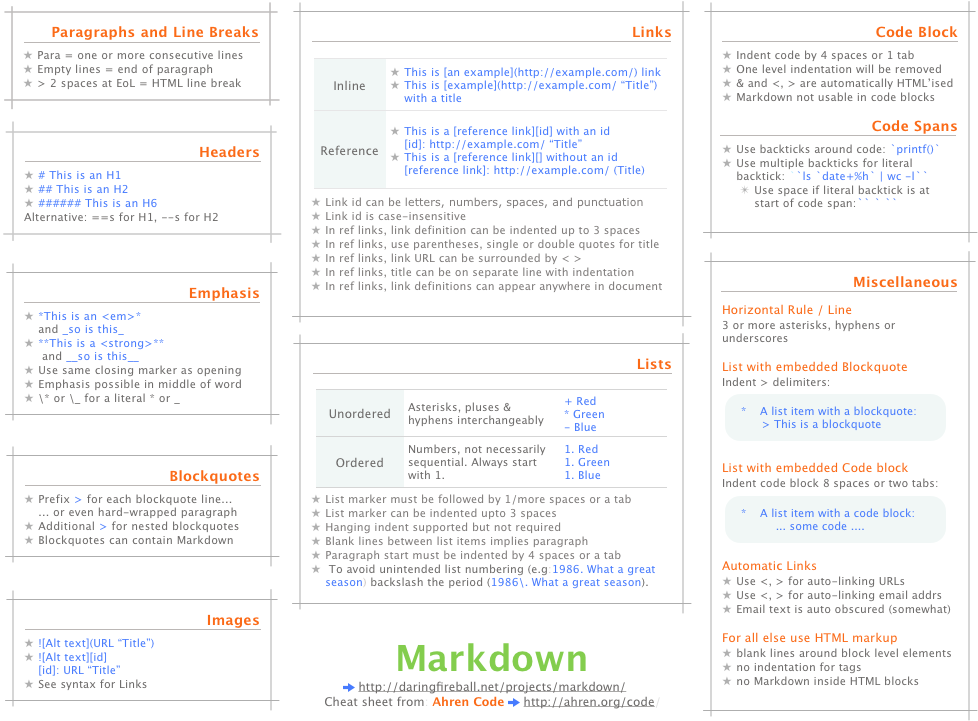
\includegraphics[width=\textwidth]{markdown_cheatsheet_02.png}
\end{figure}

\vspace{0.1in}
(三)Markdown实例
\begin{figure}[h]
  \centering
  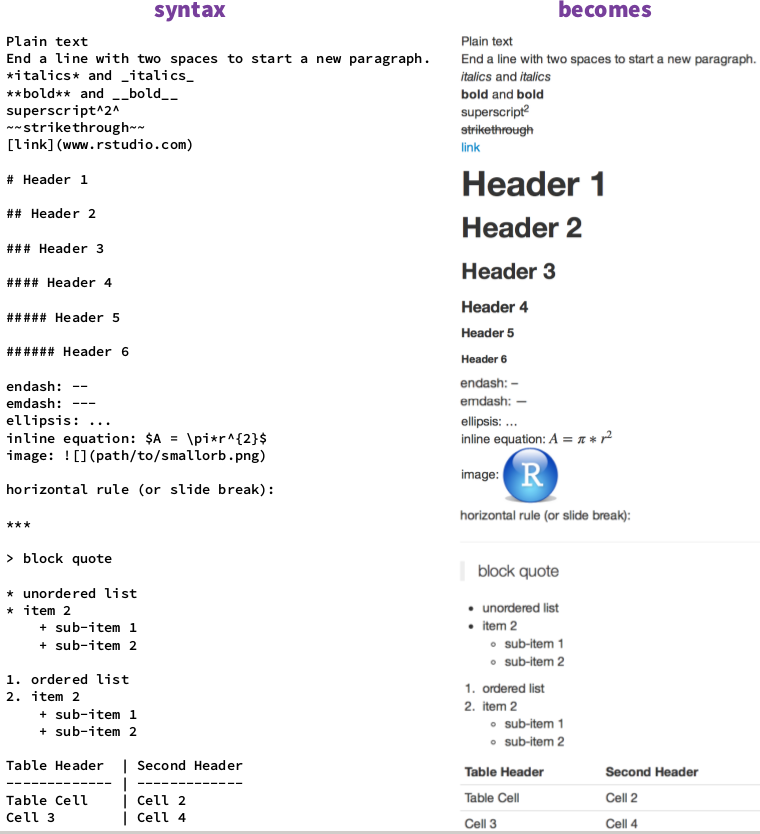
\includegraphics[width=0.8\textwidth]{markdown_example_01.png}
  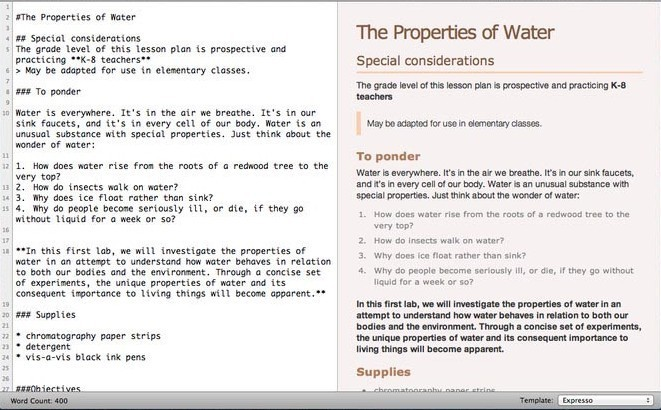
\includegraphics[width=\textwidth]{markdown_example_02.jpg}
\end{figure}

\vspace{0.1in}
(四)Markdown实践

使用Markdown撰写实验报告(日记、作业……)。
